

\tikzset{every picture/.style={line width=0.75pt}} %set default line width to 0.75pt        

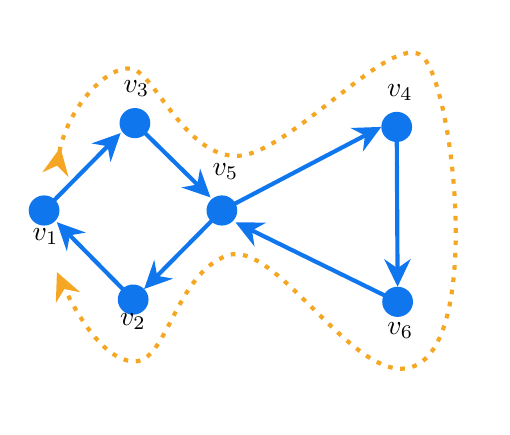
\begin{tikzpicture}[x=0.75pt,y=0.75pt,yscale=-1,xscale=1]
%uncomment if require: \path (0,178); %set diagram left start at 0, and has height of 178

%Shape: Ellipse [id:dp4798267244017467] 
\draw  [draw opacity=0][fill={rgb, 255:red, 15; green, 118; blue, 237 }  ,fill opacity=1 ] (23.01,77.75) .. controls (23.01,73.74) and (26.33,70.48) .. (30.42,70.48) .. controls (34.51,70.48) and (37.83,73.74) .. (37.83,77.75) .. controls (37.83,81.77) and (34.51,85.02) .. (30.42,85.02) .. controls (26.33,85.02) and (23.01,81.77) .. (23.01,77.75) -- cycle ;
%Shape: Ellipse [id:dp44870182967820527] 
\draw  [draw opacity=0][fill={rgb, 255:red, 15; green, 118; blue, 237 }  ,fill opacity=1 ] (65.92,120.67) .. controls (65.92,116.66) and (69.24,113.41) .. (73.33,113.41) .. controls (77.42,113.41) and (80.74,116.66) .. (80.74,120.67) .. controls (80.74,124.69) and (77.42,127.94) .. (73.33,127.94) .. controls (69.24,127.94) and (65.92,124.69) .. (65.92,120.67) -- cycle ;
%Shape: Ellipse [id:dp6247177831364052] 
\draw  [draw opacity=0][fill={rgb, 255:red, 15; green, 118; blue, 237 }  ,fill opacity=1 ] (66.76,35.66) .. controls (66.76,31.64) and (70.08,28.39) .. (74.17,28.39) .. controls (78.26,28.39) and (81.58,31.64) .. (81.58,35.66) .. controls (81.58,39.67) and (78.26,42.93) .. (74.17,42.93) .. controls (70.08,42.93) and (66.76,39.67) .. (66.76,35.66) -- cycle ;
%Shape: Ellipse [id:dp24674115427755572] 
\draw  [draw opacity=0][fill={rgb, 255:red, 15; green, 118; blue, 237 }  ,fill opacity=1 ] (108.67,77.75) .. controls (108.67,73.74) and (111.99,70.48) .. (116.08,70.48) .. controls (120.17,70.48) and (123.49,73.74) .. (123.49,77.75) .. controls (123.49,81.77) and (120.17,85.02) .. (116.08,85.02) .. controls (111.99,85.02) and (108.67,81.77) .. (108.67,77.75) -- cycle ;
%Shape: Ellipse [id:dp24305715795512062] 
\draw  [draw opacity=0][fill={rgb, 255:red, 15; green, 118; blue, 237 }  ,fill opacity=1 ] (193.33,121.75) .. controls (193.33,117.74) and (196.65,114.48) .. (200.74,114.48) .. controls (204.83,114.48) and (208.15,117.74) .. (208.15,121.75) .. controls (208.15,125.77) and (204.83,129.02) .. (200.74,129.02) .. controls (196.65,129.02) and (193.33,125.77) .. (193.33,121.75) -- cycle ;
%Shape: Ellipse [id:dp44022017328235674] 
\draw  [draw opacity=0][fill={rgb, 255:red, 15; green, 118; blue, 237 }  ,fill opacity=1 ] (192.9,37.48) .. controls (192.9,33.47) and (196.22,30.21) .. (200.31,30.21) .. controls (204.4,30.21) and (207.72,33.47) .. (207.72,37.48) .. controls (207.72,41.5) and (204.4,44.75) .. (200.31,44.75) .. controls (196.22,44.75) and (192.9,41.5) .. (192.9,37.48) -- cycle ;
%Straight Lines [id:da7847946315938599] 
\draw [color={rgb, 255:red, 15; green, 118; blue, 237 }  ,draw opacity=1 ][fill={rgb, 255:red, 0; green, 0; blue, 0 }  ,fill opacity=1 ][line width=1.5]    (30.42,77.75) -- (64.47,43.29) ;
\draw [shift={(67.28,40.45)}, rotate = 494.65] [fill={rgb, 255:red, 15; green, 118; blue, 237 }  ,fill opacity=1 ][line width=0.08]  [draw opacity=0] (13.4,-6.43) -- (0,0) -- (13.4,6.44) -- (8.9,0) -- cycle    ;
%Straight Lines [id:da4535819051227774] 
\draw [color={rgb, 255:red, 15; green, 118; blue, 237 }  ,draw opacity=1 ][fill={rgb, 255:red, 0; green, 0; blue, 0 }  ,fill opacity=1 ][line width=1.5]    (107.75,68.66) -- (74.17,35.66) ;
\draw [shift={(110.61,71.46)}, rotate = 224.5] [fill={rgb, 255:red, 15; green, 118; blue, 237 }  ,fill opacity=1 ][line width=0.08]  [draw opacity=0] (13.4,-6.43) -- (0,0) -- (13.4,6.44) -- (8.9,0) -- cycle    ;
%Straight Lines [id:da9862797560803531] 
\draw [color={rgb, 255:red, 15; green, 118; blue, 237 }  ,draw opacity=1 ][fill={rgb, 255:red, 0; green, 0; blue, 0 }  ,fill opacity=1 ][line width=1.5]    (39.37,86.22) -- (73.33,120.67) ;
\draw [shift={(36.56,83.37)}, rotate = 45.41] [fill={rgb, 255:red, 15; green, 118; blue, 237 }  ,fill opacity=1 ][line width=0.08]  [draw opacity=0] (13.4,-6.43) -- (0,0) -- (13.4,6.44) -- (8.9,0) -- cycle    ;
%Straight Lines [id:da524977452131772] 
\draw [color={rgb, 255:red, 15; green, 118; blue, 237 }  ,draw opacity=1 ][fill={rgb, 255:red, 0; green, 0; blue, 0 }  ,fill opacity=1 ][line width=1.5]    (81.44,112.72) -- (116.08,77.75) ;
\draw [shift={(78.63,115.56)}, rotate = 314.73] [fill={rgb, 255:red, 15; green, 118; blue, 237 }  ,fill opacity=1 ][line width=0.08]  [draw opacity=0] (13.4,-6.43) -- (0,0) -- (13.4,6.44) -- (8.9,0) -- cycle    ;
%Straight Lines [id:da817738331686477] 
\draw [color={rgb, 255:red, 15; green, 118; blue, 237 }  ,draw opacity=1 ][fill={rgb, 255:red, 0; green, 0; blue, 0 }  ,fill opacity=1 ][line width=1.5]    (200.31,37.48) -- (200.72,110.48) ;
\draw [shift={(200.74,114.48)}, rotate = 269.68] [fill={rgb, 255:red, 15; green, 118; blue, 237 }  ,fill opacity=1 ][line width=0.08]  [draw opacity=0] (13.4,-6.43) -- (0,0) -- (13.4,6.44) -- (8.9,0) -- cycle    ;
%Straight Lines [id:da27880354700522414] 
\draw [color={rgb, 255:red, 15; green, 118; blue, 237 }  ,draw opacity=1 ][fill={rgb, 255:red, 0; green, 0; blue, 0 }  ,fill opacity=1 ][line width=1.5]    (200.74,121.75) -- (126.2,85.22) ;
\draw [shift={(122.61,83.46)}, rotate = 386.11] [fill={rgb, 255:red, 15; green, 118; blue, 237 }  ,fill opacity=1 ][line width=0.08]  [draw opacity=0] (13.4,-6.43) -- (0,0) -- (13.4,6.44) -- (8.9,0) -- cycle    ;
%Straight Lines [id:da7034873595191173] 
\draw [color={rgb, 255:red, 15; green, 118; blue, 237 }  ,draw opacity=1 ][fill={rgb, 255:red, 0; green, 0; blue, 0 }  ,fill opacity=1 ][line width=1.5]    (116.08,77.75) -- (189.36,39.34) ;
\draw [shift={(192.9,37.48)}, rotate = 512.3399999999999] [fill={rgb, 255:red, 15; green, 118; blue, 237 }  ,fill opacity=1 ][line width=0.08]  [draw opacity=0] (13.4,-6.43) -- (0,0) -- (13.4,6.44) -- (8.9,0) -- cycle    ;
%Curve Lines [id:da5474109788589865] 
\draw [color={rgb, 255:red, 245; green, 166; blue, 35 }  ,draw opacity=1 ][line width=1.5]  [dash pattern={on 1.69pt off 2.76pt}]  (37.83,49.33) .. controls (42.44,26.79) and (61.66,7.42) .. (72.61,9.46) .. controls (83.74,11.53) and (98.46,52.15) .. (123.61,51.46) .. controls (148.76,50.78) and (198.38,-9.33) .. (212.61,3.46) .. controls (226.83,16.25) and (240.41,129.35) .. (212.61,150.46) .. controls (184.8,171.57) and (143.61,90.46) .. (118.61,99.46) .. controls (93.61,108.46) and (89.7,151.17) .. (73.61,150.46) .. controls (58.65,149.8) and (45.57,127.02) .. (38.18,110.96) ;
\draw [shift={(36.61,107.46)}, rotate = 426.37] [fill={rgb, 255:red, 245; green, 166; blue, 35 }  ,fill opacity=1 ][line width=0.08]  [draw opacity=0] (13.4,-6.43) -- (0,0) -- (13.4,6.44) -- (8.9,0) -- cycle    ;
\draw [shift={(38.27,47.37)}, rotate = 460.31] [fill={rgb, 255:red, 245; green, 166; blue, 35 }  ,fill opacity=1 ][line width=0.08]  [draw opacity=0] (13.4,-6.43) -- (0,0) -- (13.4,6.44) -- (8.9,0) -- cycle    ;

% Text Node
\draw (23.43,84.78) node [anchor=north west][inner sep=0.75pt]    {$v_{1}$};
% Text Node
\draw (65.5,126.05) node [anchor=north west][inner sep=0.75pt]    {$v_{2}$};
% Text Node
\draw (67.18,13.8) node [anchor=north west][inner sep=0.75pt]    {$v_{3}$};
% Text Node
\draw (194.16,15.62) node [anchor=north west][inner sep=0.75pt]    {$v_{4}$};
% Text Node
\draw (110.09,53.42) node [anchor=north west][inner sep=0.75pt]    {$v_{5}$};
% Text Node
\draw (194.33,130.15) node [anchor=north west][inner sep=0.75pt]    {$v_{6}$};


\end{tikzpicture}